\section{优化设计与实现}

SM4 的主要计算开销集中在 S 盒替换、线性变换、异或和循环移位上，因此本实验从三条不同思路展开优化：查表优化、指令级优化和 bit-slice 常量时间实现。

\subsection{查表优化}

SM4 的轮函数由非线性变换和线性变换构成。查表优化的核心思想是将 S 盒输出及其后续线性变换预先合并，构造成 T-table，从而用查表替代一部分重复的移位和异或操作。
这种方法属于“以空间换时间”：代价是增加约 4 KB 的查找表，收益是减少轮函数中的标量运算数量。由于实现本身不依赖 x86、ARM 或 RISC-V 专用指令，因此它属于平台无关的算法级优化。

\begin{figure}[H]
    \centering
    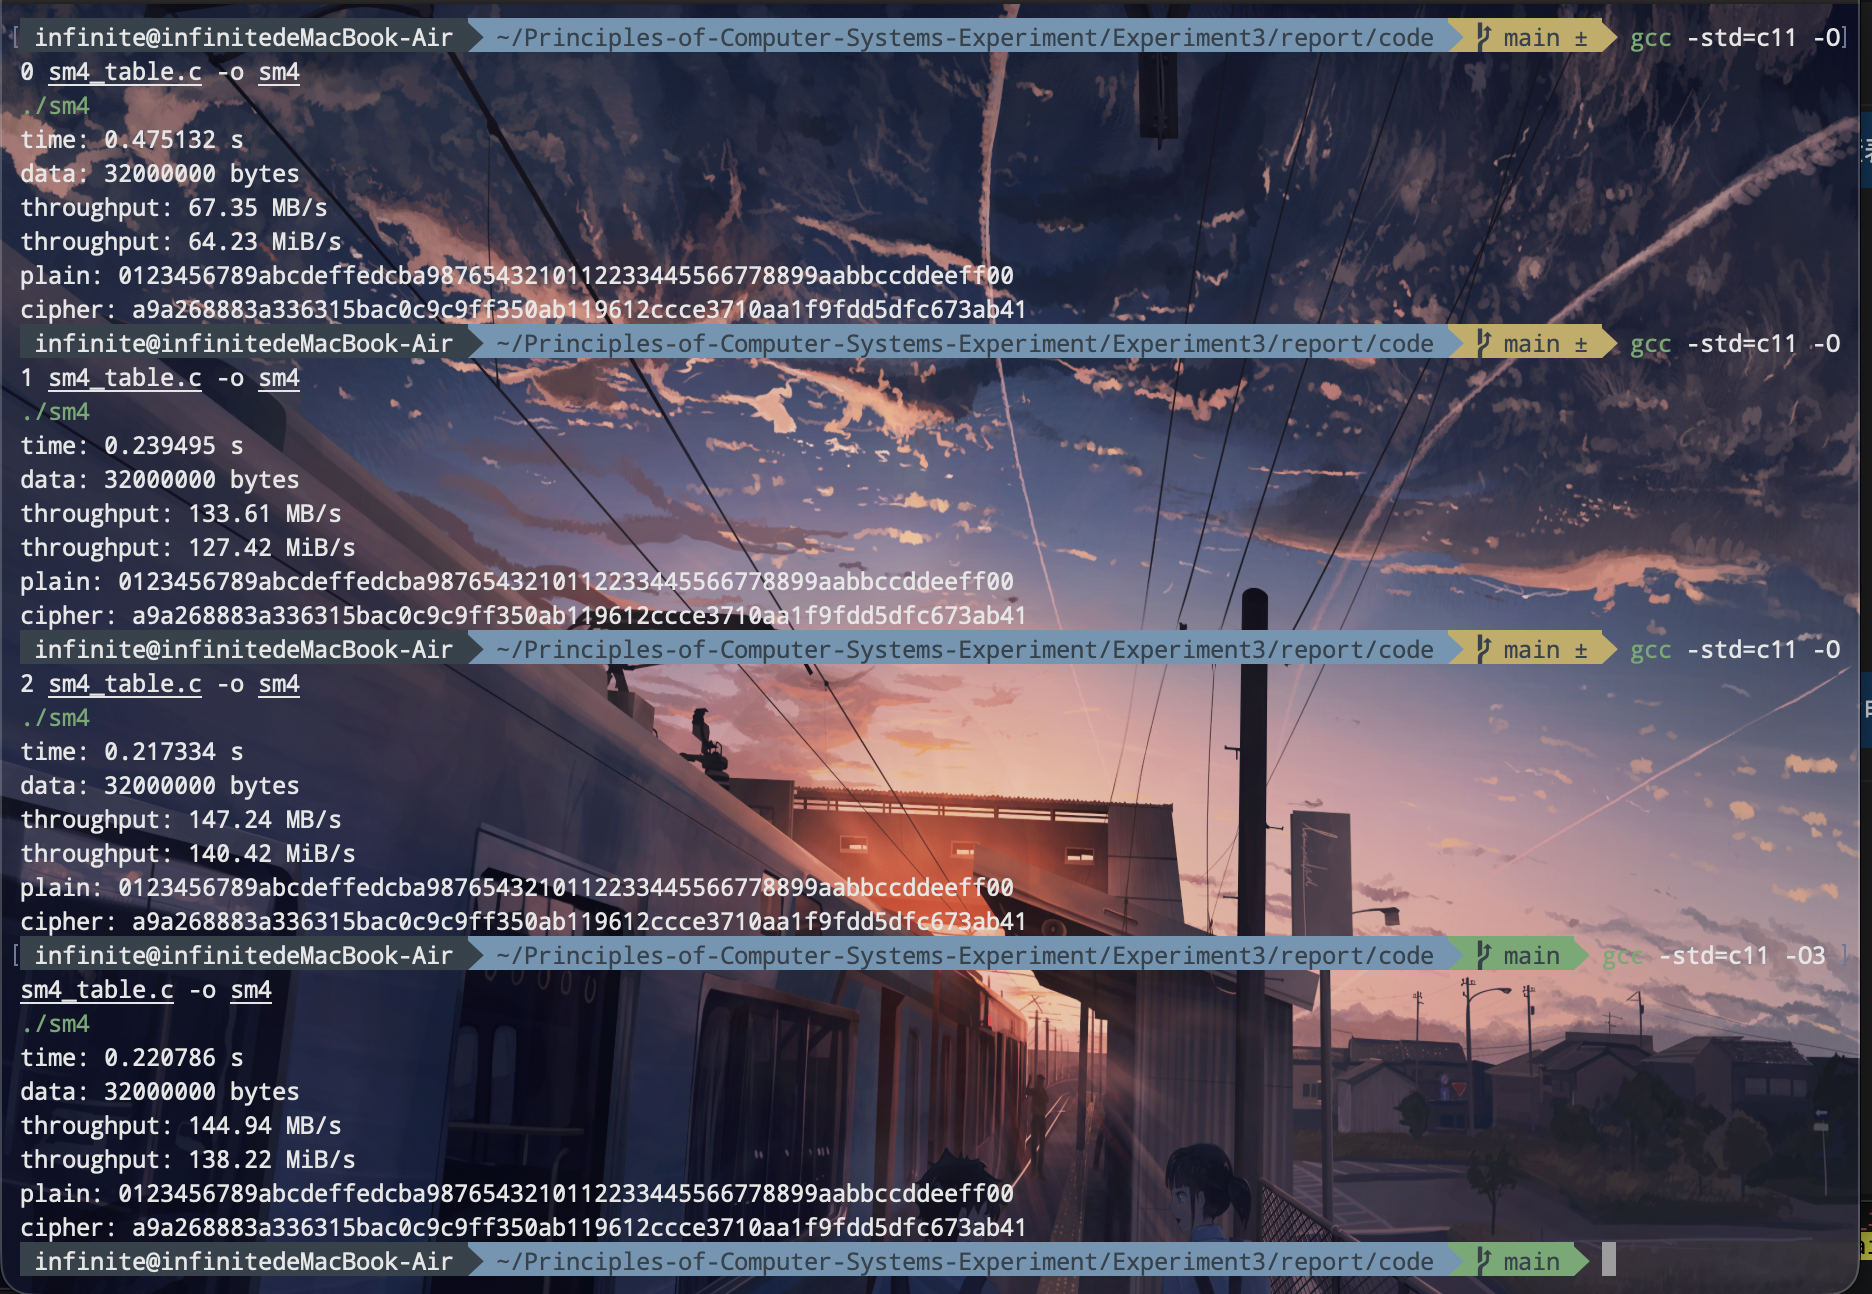
\includegraphics[width=\textwidth]{figure/table.png}
    \caption{查表优化版本的早期测试结果}
    \label{fig:sm4test_table}
\end{figure}

\begin{figure}[H]
    \centering
    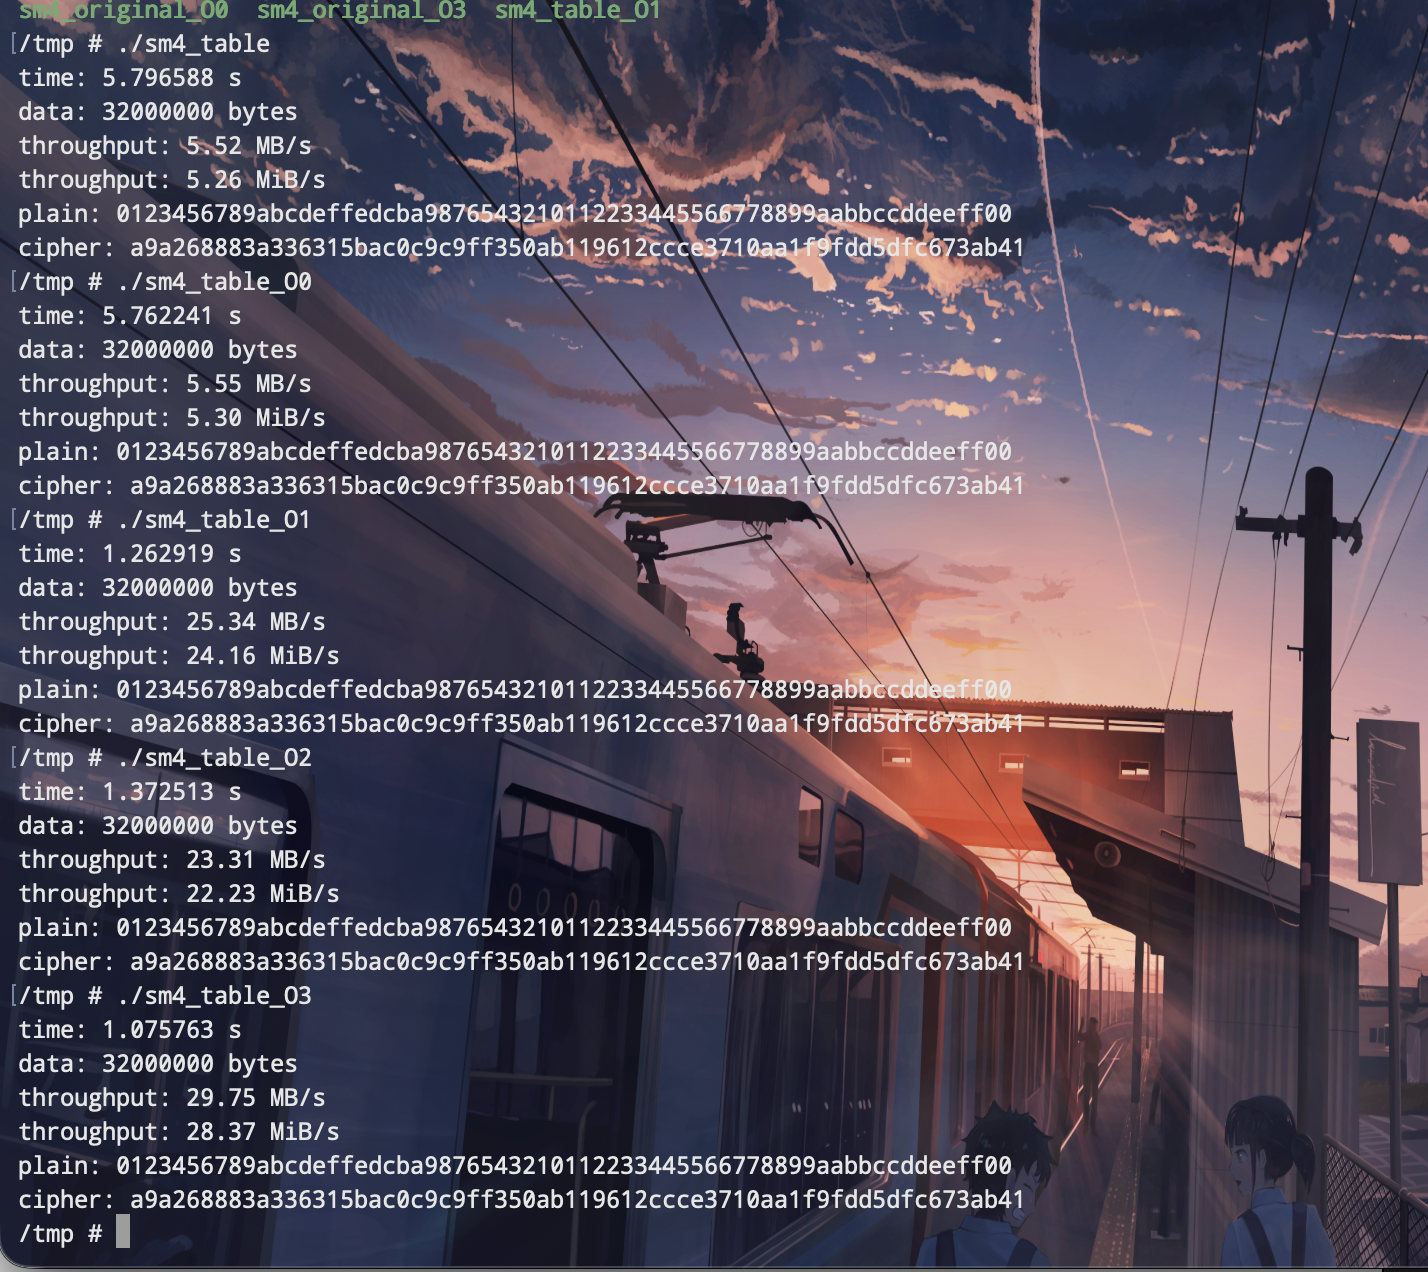
\includegraphics[width=\textwidth]{figure/riscv_table.png}
    \caption{查表优化版本在 QEMU-RISC-V 平台上的测试结果}
    \label{fig:sm4test_riscv_table_default}
\end{figure}

\subsection{指令优化}

除平台无关的查表优化外，本实验还进一步实现了 RISC-V 标量密码扩展方向的指令优化版本，即基于 Zksed 思路实现的 SM4 单数据流加密版本。该实现的目标不是改变算法结构，而是在轮函数和轮密钥生成过程中尽可能利用专用指令语义，缩短关键路径上的指令序列。

需要说明的是，在当前实验环境下，该版本运行在 QEMU 模拟器中，专用指令的潜在硬件优势会受到动态翻译开销影响，因此其性能未必显著超过查表版本。% 但从实验意义上看，这一实现已经证明了“面向 RISC-V 指令扩展的 SM4 优化”是可行的，并且确实应当被纳入本实验主线。

\subsection{SIMD 向量化优化（主机参考）}
实现基于 x86 AVX2 的 SIMD 多缓冲区版本，它能够利用 256 位向量寄存器并行处理多条独立数据流（实际上的并行），因此在主机平台上具有较高吞吐量。但这一优化强依赖 x86 的 AVX2 指令集，无法直接迁移到实际实验平台 RISC-V 中，因此只作为一种运行在主机环境中可行的优化方法。
\begin{figure}[H]
    \centering
    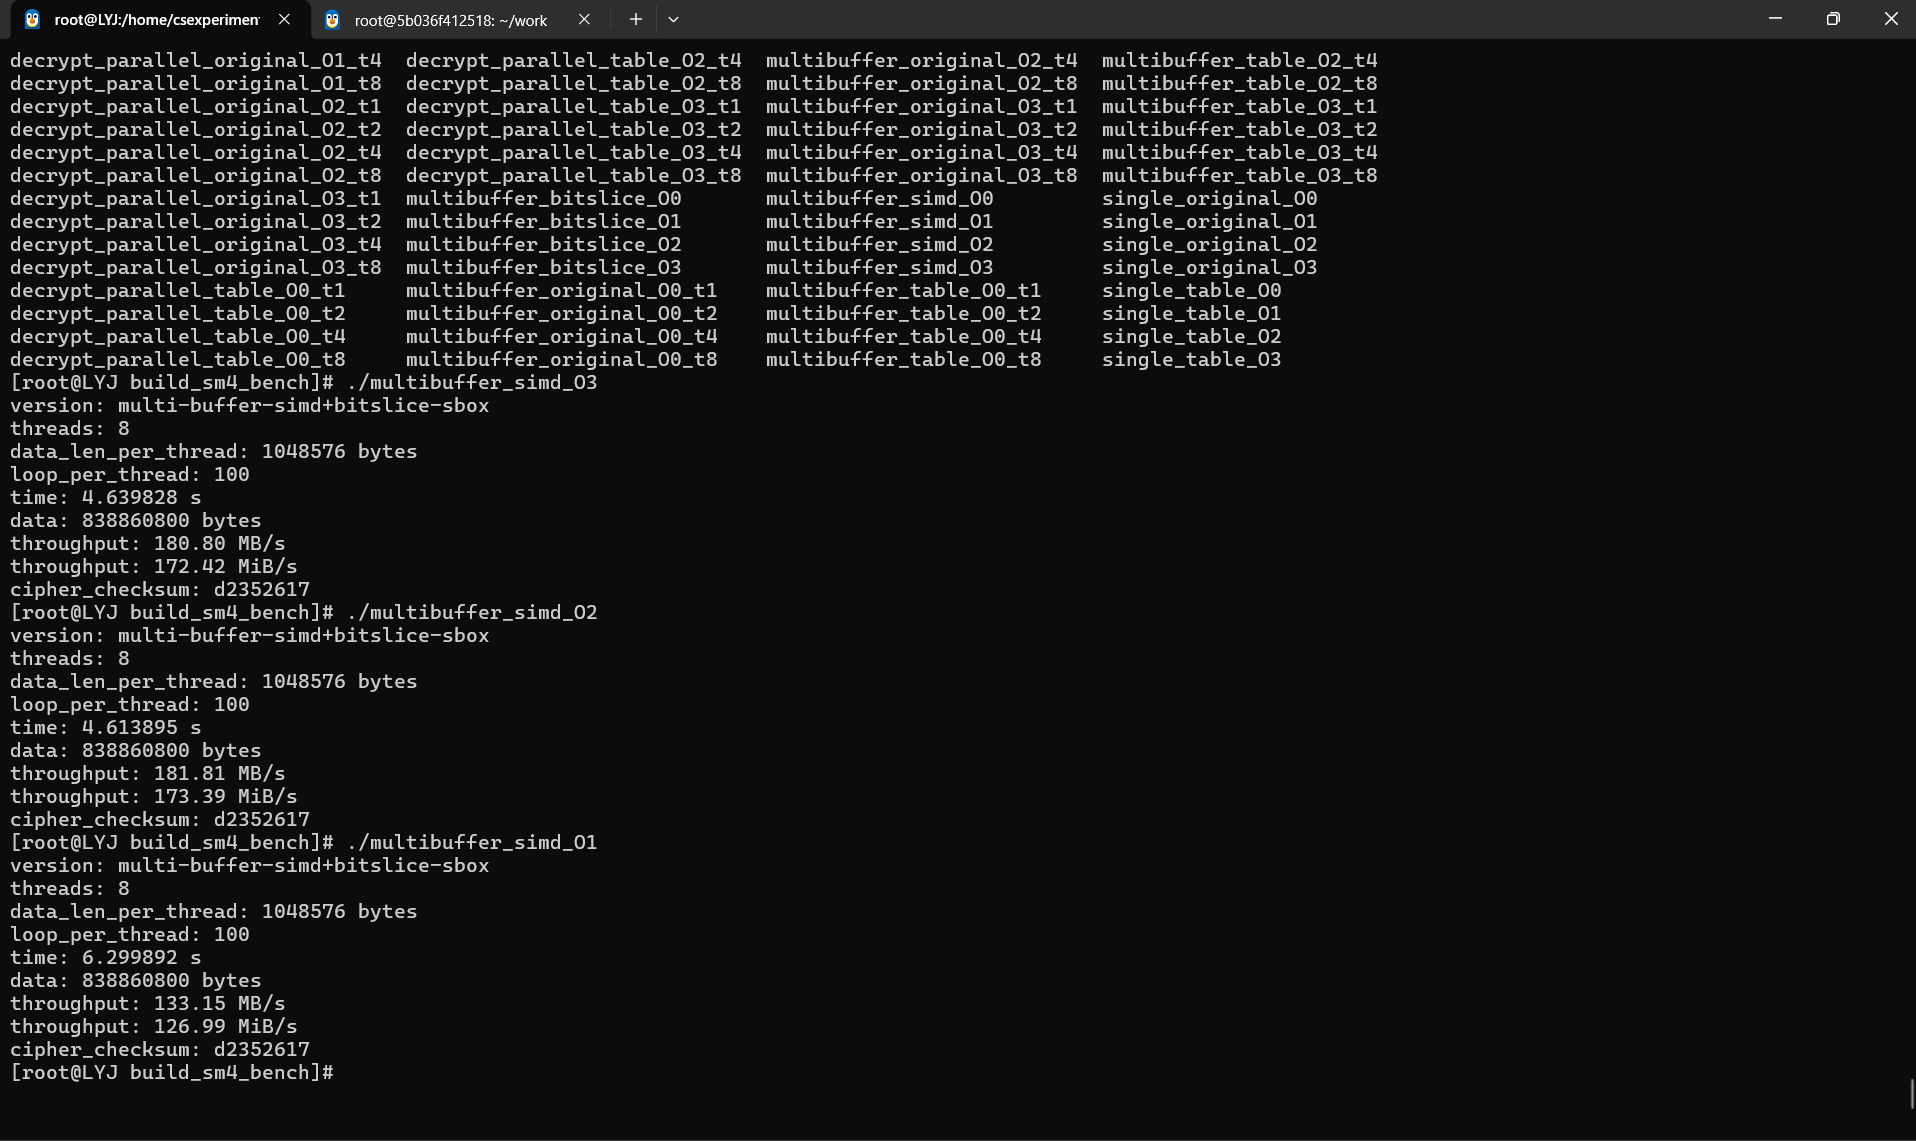
\includegraphics[width = 1\textwidth]{figure/simd_on_mainhost.png}
    \caption{SIMD优化}
\end{figure}

\subsection{Bit-Slice 常量时间实现}

bit-slice 的引入目标与查表优化不同。它并不优先追求吞吐量，而是希望用布尔逻辑门序列替代查表，从而避免与输入相关的缓存访问模式，实现更接近常量时间的执行特性。

本实验分别实现了：

\begin{enumerate}
    \item 通用 bit-slice 核心；
    \item 面向 x86 主机的 bit-slice 版本；
    \item 面向 RISC-V 平台的 bit-slice 版本。
\end{enumerate}

其中，RISC-V 版本的重点在于验证：即使不依赖 x86 SIMD 指令，也可以仅凭通用寄存器和布尔逻辑运算实现 bit-slice 形式的 SM4-CBC 计算。

但从性能角度看，bit-slice 在当前实验平台上的表现并不理想。其原因不在于实现错误，而在于布尔逻辑展开导致指令数大幅膨胀；在 QEMU 系统模拟环境中，这种膨胀会被进一步放大。因此本实验中的bit-slice作为一种更安全(抵抗测信道攻击)的优化SM4-CBC实现而非实际更高性能的优化。
